\documentclass[a4paper]{article}
\usepackage{graphicx}
\graphicspath{{./figures/}}
\usepackage[italian]{babel}
\usepackage{float}
\usepackage{braket}
\usepackage{listings}
\usepackage{mdframed}
\usepackage{tikz}
\usepackage{enumitem}
\usetikzlibrary{shapes, arrows, automata, petri, decorations.markings, decorations.pathreplacing, positioning, calc}

\usepackage{hyperref}
\hypersetup{
    colorlinks=false,
}

% Code blocks
\definecolor{codegreen}{rgb}{0,0.6,0}
\definecolor{codegray}{rgb}{0.5,0.5,0.5}
\definecolor{codepurple}{rgb}{0.58,0,0.82}
\definecolor{backcolour}{rgb}{0.95,0.95,0.95}

\lstdefinestyle{mystyle}{
	backgroundcolor=\color{backcolour},
	commentstyle=\color{codegreen},
	keywordstyle=\color{magenta},
	numberstyle=\tiny\color{codegray},
	stringstyle=\color{codepurple},
	basicstyle=\ttfamily\footnotesize,
	breakatwhitespace=false,
	breaklines=true,
	captionpos=b,
	keepspaces=true,
	numbers=left,
	numbersep=5pt,
	showspaces=false,
	showstringspaces=false,
	showtabs=false,
	tabsize=2
}

\lstset{style=mystyle}

\begin{document}

% Title ------------------------------------------------------------------------------
\title{Documentazione progetto Ingegneria del Software\\[1ex]
\large Software di gestione dei pazienti diabetici
}

\author{
\vspace{0.8cm}
Università di Verona\\
Imbriani Paolo - VR500437\\
Irimie Fabio - VR501504
}

\begin{figure}
    \centering
    
\includegraphics[width=0.3\textwidth]{UniversityofVerona}
\end{figure}

\maketitle 

\pagebreak
% Title ------------------------------------------------------------------------------

\tableofcontents

\pagebreak

\section{Requisiti e Use Case}

\subsection{Note generali}

Il software che si andrà a sviluppare è un sistema di telemedicina di un servizio clinico per la gestione
di pazienti diabetici. Gli attori principali del sistema sono i \textit{medici} (diabetologi) e i \textit{pazienti}; questi ultimi
hanno credenziali di accesso al sistema fornite dagli amministratori del servizio con cui possono autenticarsi.
Se l'autenticazione va a buon fine allora l'utente verrà indirizzato alla propria \textit{home page} in cui potrà
visualizzare le informazioni relative al loro ruolo. Nel seguente diagramma dei casi d'uso sono rappresentati
i principali attori e le loro interazioni con il sistema. Notare che diamo per scontato che tutti gli autori siano già autenticati
per semplificare il diagramma.

\begin{figure}[H]
	\centering
	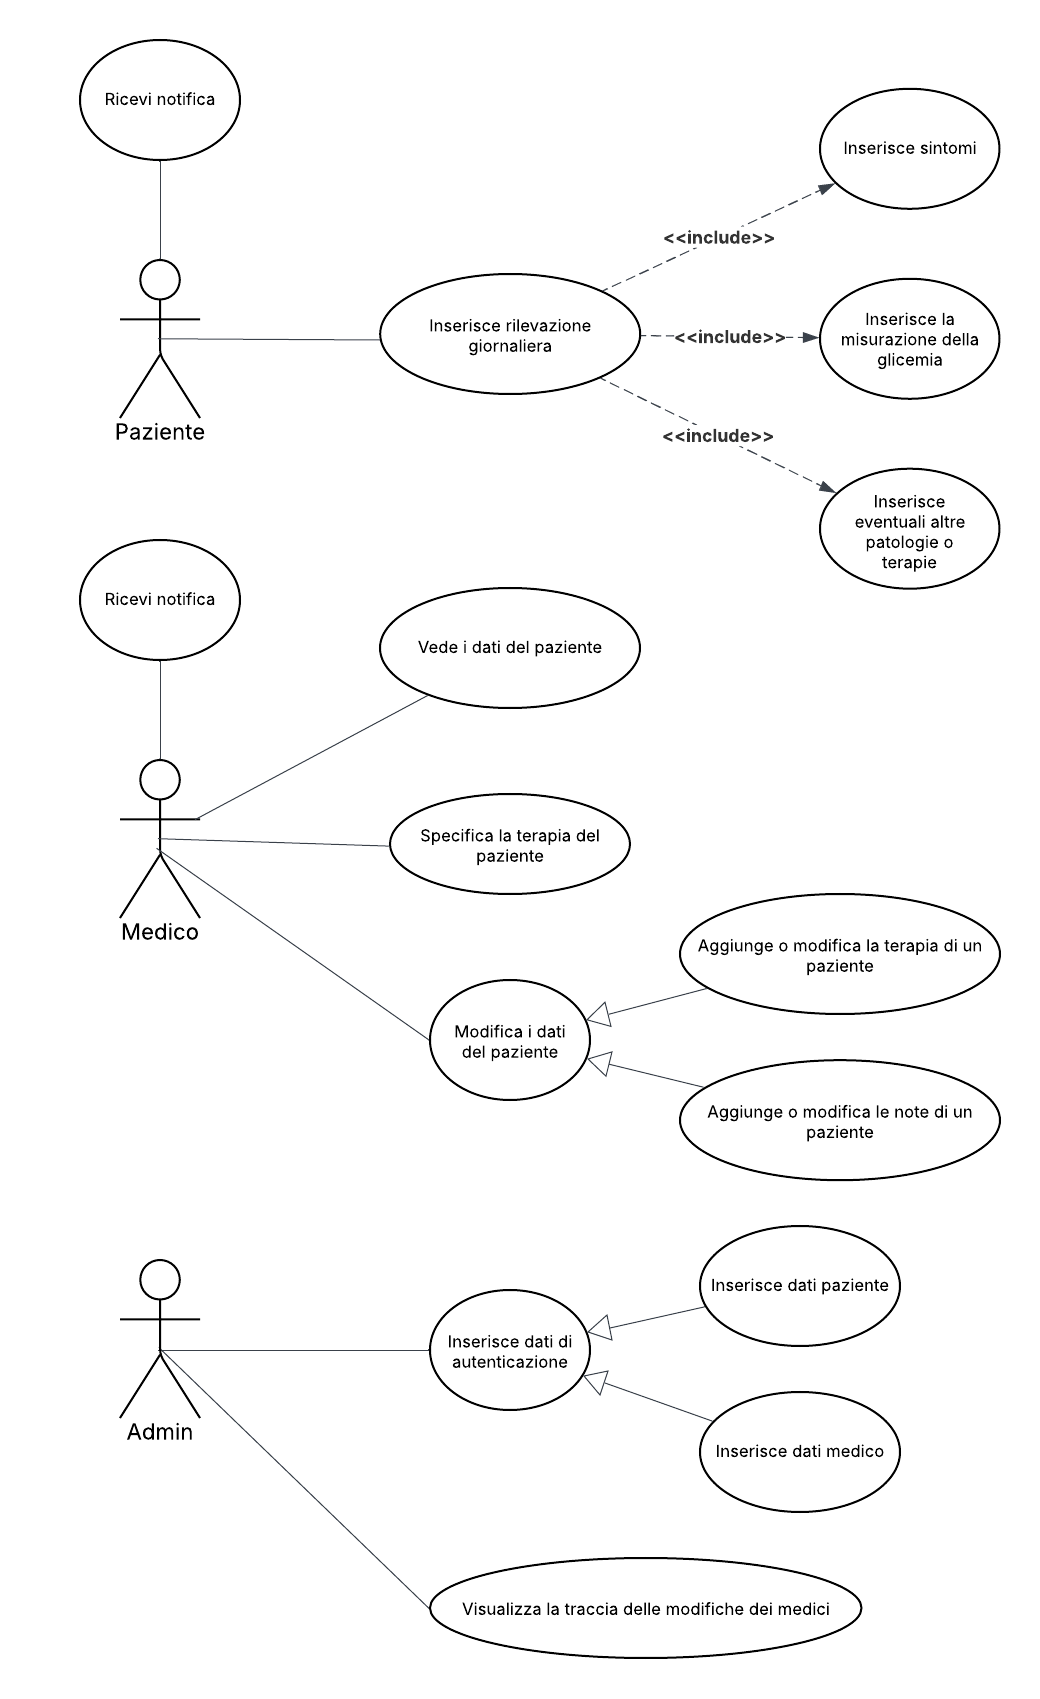
\includegraphics[width=0.7\textwidth]{usecase}
	\caption{Diagramma dei casi d'uso}
	\label{fig:usecase}
\end{figure}

\subsection{Casi d'uso del paziente}

Una volta che il paziente si è autenticato ed è entrato all'interno della sua area riservata, egli può
inserire i dati giornalieri relativi alla sua glicemia (prima e dopo ogni pasto); per fare questo
ha bisogno di inserire dati quali: sintomi, rilevazione glicemica, eventuali altre patologie o terapie.
\begin{mdframed}
  \textbf{Attore}: Paziente\\
  \textbf{Precondizioni}: Il paziente deve essere autenticato\\
  \textbf{Passi}: 
  \begin{enumerate}[nosep]
    \item Il paziente accede alla sua home page
    \item Il paziente entra dentro l'area di inserimento dei dati giornalieri
    \item  Il paziente inserisce il dato della sua glicemia prima pasto e dopo pasto
    \begin{itemize}
		\item  Il paziente può aprire un ulteriore finestra per inserire i sintomi, le terapie e le patologie, con oppurtuna data 
		\item  Può anche inserire le assunzioni di insulina o qualsiasi farmaco prescritto dal diabetologo, specificandone giorno, ora, farmaco e quantità assunta
	\end{itemize}
	\item Il paziente inserisce la data e ora di rilevazione
	\item Il paziente conferma l'inserimento dei dati
  \end{enumerate}
  \textbf{Postcondizioni}: La rilevazione è inserita 
\end{mdframed}
\noindent
Andiamo a specificare come viene gestito l'inserimetno dei dati del paziente: i dati glicemici sono quelli
che il paziente inserisce giornalmente e obbligatori per inviare la rilevazioni. Dopo aver inserito i dati ha due possibili opzioni:
\begin{itemize}
	\item Inserimento all'interno di un textbox della patalogia, terapia o sintomi che il paziente sta avendo in quel momento
	\item La possibilità di inserire le assunzioni di insulina o qualsiasi altro farmo prescritto dal diabetologo (data, ora, farmaco, quantità) 
\end{itemize}
Le rilevazioni possiedono un ID univoco che le identificano inequivocabilmente e sono associate ad un paziente.

\begin{figure}[H]
	\centering
	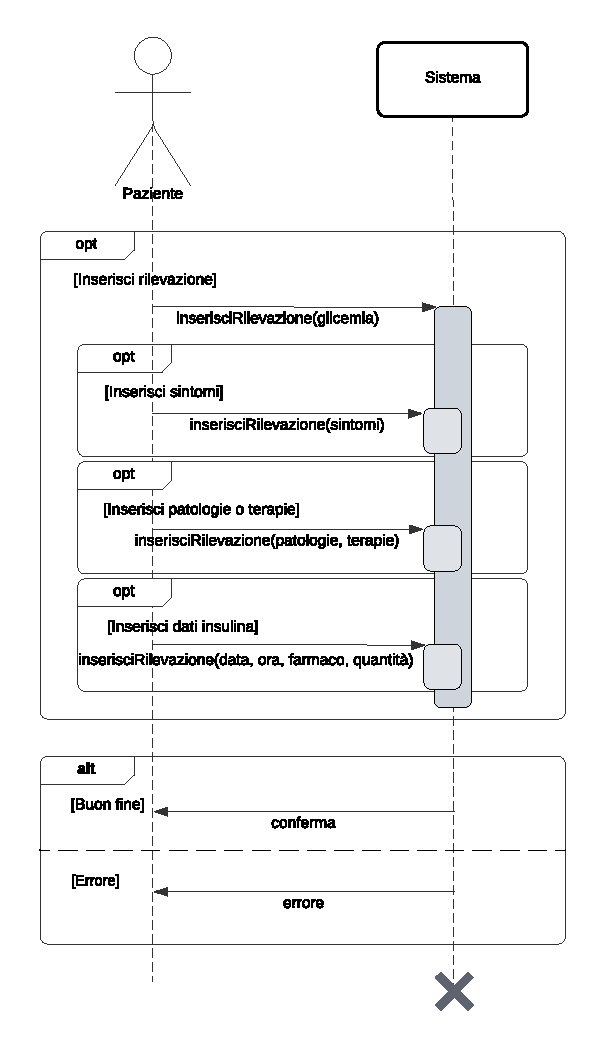
\includegraphics[width=0.7\textwidth]{sdPaziente}
	\caption{Sequence Diagram della rilevazione del paziente}
	\label{fig:usecase}
\end{figure}

\end{document}
